% !TEX root = mainthesis.tex
%Chapter 4

\renewcommand{\thechapter}{4}

\chapter{Manipulation and detection of ultra-cold atoms}
\label{ch:Ch3}

All of our experiments rely on the interaction of atoms with electric and magnetic fields, both for the preparation of ultra-cold atoms through laser cooling and trapping, for the engineering of interesting Hamiltonians, and for detection. In this chapter I will first describe the electronic structure of $\Rb87$ which makes all of our experiments possible and then I will review the effects of the magnetic and electric interactions that are relevant to our experiments. I will not cover laser cooling which has been covered extensively in the literature (see~\cite{metcalf_deceleration_1999} for example). 

\section{Electronic structure of $^{87}$Rb}
\label{sec:electronic_structure}

Rb is an Alkali metal (also Li, which exists in our vacuum chamber but was never used). Alkali metals correspond to the first group (leftmost column) of the periodic table and are characterized by having a single valence electron, which makes the description of their internal structure much simpler than that of other elements. In genera we can describe the state of an electron in an atom by it's angular momentum $\mathbf L$ and its spin $\mathbf{S}$. Because of Pauli's exclusion principle there can not be two electrons with the same quantum numbers and in multi-electron atoms they tend to fill `shells' of different angular momentum values, historically labeled by the letters $S,\ P,\ D,\ F,\ ...$\footnote{This terms were used to describe the lines in the emission spectra when they were first discovered. $S$ stands for sharp, $P$ for principal $D$ for diffuse and $F$ for further noted} (corresponding to $\mathbf{L}=1,\ 2,\ 3,\ 4,\ ...$). In particular Rb has 4 filled shells and one electron in the $5S$ 
shell (the number $5$ corresponds to the principal quantum number). Figure~\ref{fig:fs_hfs}a shows the energy levels of a $5S$ and $5P$ orbital.

The atomic level structure is modified by a fine structure splitting of the electronic orbitals into levels with different total electronic angular momentum $\mathbf{J}=\mathbf{L}\cdot\mathbf{S}$. This effect  arises from a spin-orbit interaction between the electron's spin and orbital angular momentum $\hat H_{fs} \propto \mathbf{L}\cdot\mathbf{S}$. Figure~\ref{fig:fs_hfs}b show the $5^2S_{1/2}$, $5^2P_{1/2}$ and $5^2P{3/2}$ electronic configurations that arise from this splitting.  The atomic level structure gets further modified by the nuclear spin $\mathbf{I}$ which interacts with the electron's intrinsic magnetic flux density through the magnetic dipole interaction to give rise to the hyperfine splitting. For $S$ electrons the hyperfine splitting can be described by the Hamiltonian $\hat H_{hfs} = A_{hfs}\mathbf{I}\cdot\mathbf{J}$\footnote{Notice how both the fine and hyperfine structure arise from a spin-orbit coupling interaction, we will discuss a very different type of spin-orbit coupling in future chapter.}. Figure~\ref{fig:fs_hfs}c shows the fine structure getting further split into states of total angular momentum $\mathbf{F}=\mathbf{J}+\mathbf{I}$. $\Rb87$ has a nuclear spin $I=3/2$ and therefore its ground state hyperfine configuration has $F=1$ and $F=2$. 


\note{Something about what we use this transitions for and how we usually ignore all other levels. (???)}

\note{TODO: what about matrix elements between -1 and +1?. Move to intro chapter}

\section{Magnetic interaction}
\subsection{Static magnetic fields}
Also talk about the Paschen–Back effect occurs in a strong external magnetic field. The spin and orbital angular momen- tum precess independently about the magnetic field.

Uniform fields: Zeeman splitting, Breit-Rabi formula
Gradients: Quadrupole potentials and Stern-Gerlach

\subsection{Oscillatory magnetic fields}
\label{seq:rf_coupling}
RF coupling and microwave coupling

\subsection{Selection rules}

\section{Applications}
\subsection{Quantum coherent dynamics?}
\subsection{Adiabatic rapid pasage}
\label{sec:arp}
\subsection{The Rabi cycle}
\subsection{Ramsey interferometry}


\section{Atom-light interaction}
In the presence of an electric field $\mathbf E$ an atom can become polarized and therefore it's energy levels get shifted through the Stark effect~\cite{stark_beobachtungen_1914}. If the electric field is spatially uniform with respect to the atom's size the effect of the electric field on the atom can be described by the the Hamiltonian   
%
\begin{equation}
\hat{H} = -\mathbf{\hat d}\cdot\mathbf{E},
\label{eq:dipole_ham}	
\end{equation}
%
where $\mathbf{\hat d}=-e\sum_j r_j$ is the atomic dipole operator, $e$ is the electron charge and $\hat r_j$ are the position operators of the atom's electrons relative to the center of mas of the atom. This approximation, known as the dipole approximation, treats the atom as a quantum object and the electric field as a classical object. Here I will only consider the case of oscillating electric fields $\mathbf{E}=E_0\cos(\omega t)\boldsymbol{\epsilon}$ (i.e. plane waves of electromagnetic radiation) which are relevant to our experiments. 

Can break interaction into scalar, vector and tensor part. Interaction can also be resonant or off-resonant.

\note{Why do you only get second order perturbation theory effects? I think it has something to do with unperturbed atomic states being eigenstates of the parity operator}

% \subsection{Scalar light shift: Dipole traps and optical lattices}

% \subsection{Vector light shift: Raman coupling}



\subsection{Light induced spin-orbit coupling}

The geometry and wavelength of the Raman fields determine the natural units of the system: the single photon recoil momentum $k_{\mathrm{L}}=\sqrt{2}\pi/\lambda_{\mathrm{R}}$ and its associated recoil energy $E_{\mathrm{L}}=\hbar^2k_{\mathrm{L}}^2/2m$, as well as the direction of the recoil momentum $\mathbf{k}_{\mathrm{L}}=k_{\mathrm{L}}\ex$. The Raman wavelength was $\lambda_{\mathrm{R}}=790.032\,\nm$, as usual, so that the scalar light shift is zero. 

\section{Rashba SOC in condensed matter}

% In earlier sections we discussed the spin-orbit coupling interaction between spin and angular momentum that gives rise to the atomic level structure. In condensed matter systems, there is another kind of spin-orbit coupling that links the spin of the electrons with the linear or crystal momentum. In 2D materials, SOC can be represented as a sum of Rashba~\cite{bychkov_oscillatory_1984} and Dresselhaus~\cite{dresselhaus_spin-orbit_1955} SOC. 

Rashba SOC~\cite{bychkov_oscillatory_1984} appears in condensed matter systems where electrons are confined in a 2D plane and experience an intrinsic out-of-plane electric field. If the electron's momentum is given by $\hbar\k=\hbar(k_x\ex+k_y\ey)$ and the electric field is $\mathbf{E}=E\ez$, in the electron's moving frame there will be a momentum dependent magnetic field $\mathbf{B}_{\rm SOC}=-\hbar\k/m\times\mathbf{E}/c^2=\hbar E/mc^2(-k_y, k_x, 0)$. The interaction between the electron's spin with this field through the magnetic Zeeman interaction $-\mathbf{\mu}\cdot{\mathbf{B}_{\rm SOC}}$ gives rise to the SOC Hamiltonian
%
\begin{equation}
	\hat{H}_{\rm SOC}=\frac{2\alpha}{m}(k_y\hat{\sigma}_x-k_x\hat{\sigma}_y)
	\label{eq:Rashba_ham}
\end{equation}
%
where $\alpha=g\mu_BE/c^2$, $g$ is the electrons gyromagnetic ratio, $\mu_B$ is the Bohr magneton and $\hat{\sigma}_i$ are the Pauli matrices. 

The Rashba dispersion relation is characterized by having a Dirac point located at $\k=0$ (see Chapter~\ref{sec:2_level_topology}) and a degenerate ground state that is described by the ring $k_x^2+k_y^2=\alpha^2$. \note{TODO: Make figure}

The Rashba Hamiltonian when combined with the free particle Hamiltonian can be interpreted as a non-abelian gauge potential. This comes from the fact that the Hamiltonian can can be written as $\hat{H}=(\hbar\k-\hat{\mathbf{A}})^2/2m$ where $\mathbf{\hat{A}}=\alpha(\hat{\sigma}_y\ex-\hat{\sigma}_x\ey)$ can be interpreted as a matrix valued vector potential or non-abelian gauge potential whose elements do not commute. This term is closely related to the Berry connection discussed in Chapter~\ref{sec:Berry phase and curvature}. 


\section{Rashba SOC for neutral atoms}
\label{sec:rashba_ring_coupling}

Proposals for engineering Rashba type SOC in neutral atoms consist in using lasers to link internal states of an atom with its linear momentum.
In order to achieve non-trivial gauge potentials it is necessary to couple $N\geq3$ levels (see~\cite{goldman_light-induced_2014}). We follow the proposal by~\cite{campbell_realistic_2011} which considers a `ring coupling' which is shown in Figure~\ref{fig:rashba_ring_coupling} for the case of $N=3$. The states $\ket{j}$ represent internal atomic states and they are linked to each other with complex valued matrix elements $\frac{\Omega_j}{2}e^{i\k_{j}\cdot\x}$, where $\k_{j}$ is a momentum transfer associated with the $\ket{j}\rightarrow\ket{j+1}$ transition and $\Omega_i=e^{i\phi_i}\vert\Omega\vert$ represents the coupling strength. We require that $\sum\k_i=0$ so that no momentum is transfered when a closed loop $\ket{1}\rightarrow\ket{2}\dots \rightarrow\ket{N}\rightarrow\ket{1}$ is completed. For this case the $\k_i$ momenta vectors can be written as $\k_j=\mathbf{K}_{j+1}-\mathbf{K}_j$, and we make $\mathbf{K}_j=\kl\sin(2\pi j/N)\ex+\kl\cos(2\pi j /N)\ey$, corresponding to the vertices of an N sided regular polygon. We can further make a gauge transformation such that we can replace the phases $\phi_i$ associated to each coupling with $\bar{\phi}=\sum_i\phi_i/N$.

\begin{figure*}[htb]
\begin{center}
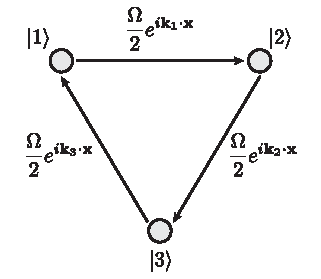
\includegraphics[]{Figures/Chapter8/Rashba_ring_coupling.pdf}
\caption[The Rashba ring coupling]{The Rashba ring coupling. To generate Rashba SOC in a system of cold atoms it is necessary to cyclically couple $N\geq3$ internal states such that the transition $\ket{j}\rightarrow\ket{j+}1$ has a momentum transfer $\k_j$ and $\sum_j\k_j=0$ such that there is no momentum transfer for a closed loop $\ket{1}\rightarrow\ket{2}\dots\ket{N}\rightarrow\ket{1}$. The ring coupling combined with the free particle Hamiltonian give rise to a 2-level subspace that can be described to first order by the Rashba Hamiltonian}
%
\label{fig:rashba_ring_coupling}
\end{center}
\end{figure*}
%
The Hamiltonian describing this coupling along with the kinetic term is 
%
\begin{equation}
	H_{j, j'}=\frac{\hbar^2 k^2}{2m}\delta_{j,j'} + \frac{\Omega}{2}(e^{i(\bar{\phi}+\k_j\cdot\x)}\delta_{j, j'+ 1} + {\rm h.c.}),
\end{equation}
%
and after applying the unitary transformation $U_{j, j'}=\exp[i\mathbf{K}_i\cdot\x]\delta_{j,j'}$\footnote{This transformation is equivalent to applying a state dependent momentum boost $\k\rightarrow \k +\mathbf{K}_j $} it gets transformed to 
%
\begin{equation}
	H_{j,j'}=\frac{\hbar^2}{2m}\vert \q +\mathbf{K}_j\vert^2\delta_{j,j'} + \frac{\Omega}{2}(e^{i\bar{\phi}}\delta_{j, j'+ 1} + {\rm h.c.}),
	\label{eq:rashba_tight_binding}
\end{equation}
%
where we have replaced the momentum $\k$ by the quasimomentum $\q$. The off diagonal terms of Equation~\ref{eq:rashba_tight_binding} can be related to a 1D periodic tight-binding Hamiltonian with hopping elements $\Omega/2$ where the internal states $\ket{j}$ represent lattice sites and completing one loop corresponds to gaining a `flux' of $N\bar{\phi}$. It is helpful to write the Hamiltonian in a basis that is conjugate to the index $j$
%
\begin{equation}
	\ket{l}=\frac{1}{\sqrt{N}}\sum_{j=1}^N e^{i2\pi jl/N}\ket{j}
\end{equation}
%
where the index $l$ is analogous to the crystal momentum index for a Bloch Hamiltonian. In this new basis, terms with oscillatory components (e.g. $\vert \q + \mathbf{K}_j\vert$) in the diagonals are displaced to the off-diagonal and oscillatory terms in the off diagonal are displaced to the diagonal. Under this basis the Hamiltonian starts looking very much Rashba-like
%
\begin{equation}
	H_{l,l'} = \left[\frac{\hbar^2}{2m}(q^2+ k_L^2)+E_l\right]\delta_{l,l'} + \frac{\hbar^2\kl}{m}\left[(iq_x+q_y)\delta_{l-1,l'}+{\rm h.c}\right],
	\label{eq:ring_coupling_ft}
\end{equation}
%
where $E_L=2\hbar\Omega\cos(2\pi l/3+\bar{\phi})$ correspond to the eigenenergies when $q=0$. The phase $\bar{\phi}$ can be tuned such that a pair of states with consecutive $l$ index become degenerate, indicating the presence of a Dirac point at $q=0$. Figure~\ref{fig:ring_coupling_energies} shows the energies $E_l$ for $N=3$ and $\bar{\phi}=0$.

\begin{figure*}[htb]
\begin{center}
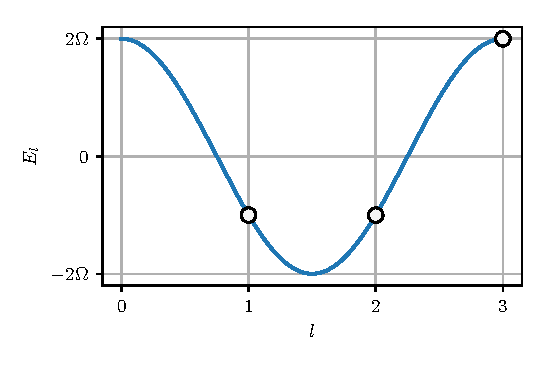
\includegraphics[]{Figures/Chapter8/ring_coupling_energies.pdf}
\caption[Rashba ring coupling eigenenergies]{Eigenenergies of Equation~\ref{eq:ring_coupling_ft} for $q=0$ for $N=3$ and $\bar{\phi}=0$. For this particular choice of phase, the energies of the $l=1$ and $l=2$ states become degenerate}
\label{fig:ring_coupling_energies}
\end{center}
\end{figure*}

We consider the degenerate states corresponding to two consecutive $\ket{l}$ states as pseudospins which are described to zeroth order by the Rashba plus free particle Hamiltonian
%
\begin{equation}
	\hat{H}^{(0)} = \frac{\hbar^2q^2}{2m} + \frac{\hbar^2\kl}{m}(\hat{\sigma_x}q_y-\hat{\sigma}_yq_x), 
\end{equation}
 %
with spin orbit coupling strength given by $\alpha=\hbar^2k_L/2$. The zeroth-order Hamiltonian has continuous rotational symmetry while we the proposed ring coupling only has only discrete rotational symmetry. The symmetry of the Hamiltonian is recovered when higher order corrections of the Hamiltonian are included. The complete expressions for the higher order terms for $N=3$ and $N=4$ can be found in~\cite{campbell_realistic_2011}, and they are reminiscent of quadratic and cubic Dresselhaus SOC~\cite{stanescu_spin_2007}. The largest leading order term is inversely proportional to $\Omega^2$ so that this ring-coupling scheme results in a more `Rashba-like' Hamiltonian as one goes to higher coupling strengths. Figure~\ref{fig:rashba_alien} shows level curves of the ground state eigenenergies of Equation~\ref{eq:ring_coupling_ft} for $N=3$ and $\bar{\phi}=0$ for increasing $\Omega$. At low $\Omega$ the dispersion has discrete rotational symmetry and is characterized by three local minima. As $\Omega$ is increased the local minima start merging into each other and in the large $\Omega$ limit we recover the characteristic Rashba ring-like dispersion.   

\begin{figure*}[htb]
\begin{center}
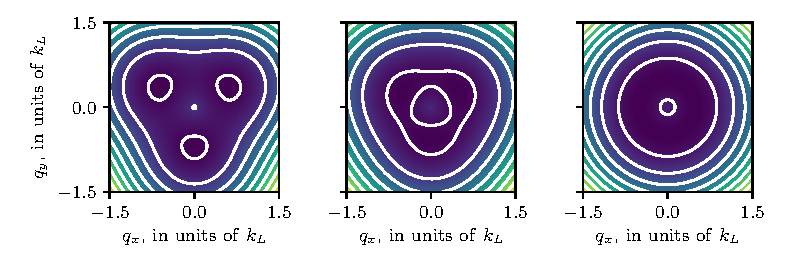
\includegraphics[]{Figures/Chapter8/rashba_alien.pdf}
\caption[Rashba ring coupling ground state dispersion]{Ground state dispersion relation of Equation~\ref{eq:ring_coupling_ft} for $N=3$ and $\bar{\phi}=0$ for $\Omega=\unit[1.75]{\El}$ (left), $\Omega=\unit[3.5]{\El}$ (middle) and $\Omega=\unit[175]{\El}$ (right). Higher order corrections to $\hat{H}^{(0)}$ decay as $1/\Omega^2$ and in the large $\Omega$ limit we recover the Rashba ring dispersion.}
\label{fig:rashba_alien}
\end{center}
\end{figure*}

So far we have only considered the case where all the coupling strengths and the vectors $\k_j$ are symmetric. In the lab it might be hard due to constraints imposed by the capabilities of an experimental apparatus. As one departs from the ideal ring-coupling, we find that the resulting dispersion can looses its discrete rotational symmetry. While this perturbations can have a significant impact on the dispersion, the Dirac point is remarkably robust and as long as $\bar{\phi}$ is such that there are at least two degenerate states in the ideal ring coupling case the Dirac point will remain gapless although it might move from $\q=0$. The exact location of the Dirac point as a function of $\Omega_i$ and $\q$ for an imperfect ring-coupling scheme is derived in \cite{huang_experimental_2016}. Figure~\ref{fig:rashba_perturbed} shows some examples of how the ground state dispersion is modified when the vectors $\mathbf{K}_j$ that don't lie in the vertices of a regular polygon and when the amplitude of $\Omega$ is state dependent. 

\begin{figure*}[htb]
\begin{center}
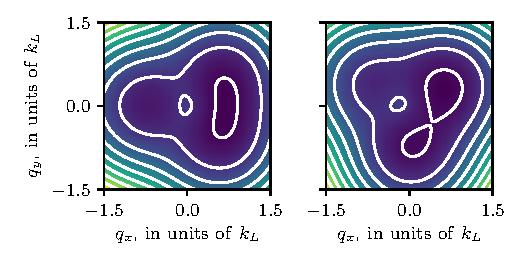
\includegraphics[]{Figures/Chapter8/rashba_perturbed.pdf}
\caption[Perturbed Rashba dispersion]{(left) Ground state dispersion relation of Equation~\ref{eq:ring_coupling_ft} for $N=3$ and $\bar{\phi}=0$ for $\Omega=\unit[1.75]{\El}$ but $\mathbf{K}_j$ that don't correspond to to the vertices of an isosceles triangle rather than an equilateral triangle. Ground state dispersion for symmetric $\mathbf{K}_j$ but state dependent $\Omega=$. In both cases the discrete rotational symmetry is lost but the gapless Dirac point remains.}
\label{fig:rashba_perturbed}
\end{center}
\end{figure*}


\section{Absorption imaging}
\subsection{Time of flight imaging}
\subsection{Partial transfer absorption imaging: magnetic field stabilization}
\label{sec:ptai}
We then apply a pair of $250\,\mu\mathrm{s}$ microwave  pulses that each transfer a small fraction of atoms into the $5^2{\rm S}_{1/2}$ $f=2$ manifold that we use to monitor and stabilize the bias field \cite{leblanc_direct_2013}. The microwave pulses are detuned by $\pm 2\, \kHz$ from the $\ket{f=1,m_F=0}\leftrightarrow\ket{f=2,m_F=1}$ transition and spaced in time by $33\, \mathrm{ms}$ (two periods of $60\, \mathrm{Hz}$). We imaged the transferred atoms following each pulse using absorption imaging\footnote{We did not apply repump light during this imaging, so the untransferred atoms in the $f=1$ manifold were largely undisturbed by the imaging process.}, and count the total number of atoms $n_1$ and $n_2$ transferred by each pulse. The imbalance in these atom numbers $(n_1-n_2)/(n_1+n_2)$ leads to a $4\kHz$ wide error signal that we use both to monitor the magnetic field before each spectroscopy measurement and cancel longterm drifts in the field. 
\section{Floquet}
\label{sec:Floquet_theory}
How to treat systems when RWA is not valid and how to create new effective (stroboscopic) Hamiltonians.
